\documentclass[12pt,fleqn]{beamer}
%\usetheme{Szeged}
\usepackage[utf8]{inputenc}
\usepackage{amsmath}
\usepackage{amsfonts}
\usepackage{amssymb}
\usepackage{lmodern}
\usepackage{listings}
\usepackage[T1]{fontenc}
\usepackage{tikz}
\usetikzlibrary{arrows,matrix}
\tikzset{>=stealth,font=\scriptsize}

\DeclareMathOperator{\dom}{dom}
\DeclareMathOperator{\cod}{cod}
%\DeclareMathOperator{\ker}{ker}
%\DeclareMathOperator{\hom}{hom}

\author{Keith A. Lewis}
\title{Category Theory}
%\setbeamercovered{transparent} 
%\setbeamertemplate{navigation symbols}{} 
%\logo{} 
%\institute{} 
%\date{} 
%\subject{} 
\begin{document}

\begin{frame}
\titlepage
\end{frame}

\begin{frame}
\begin{itemize}
\item Invented in the 40's by Eilenberg and Mac Lane to unify and generalize common constructions in algebraic topology.

\item If mathematics is abstract nonsense, then Category Theory
is generalized abstract nonsense. {\em Every proof is a put-on,
or its dual, a push-over.}

\item Computer scientists find it useful for rigorously reasoning
about programs and algorithms. E.g., Horner's rule
is a catamorphism.
\end{itemize}
\end{frame}

%\begin{frame}
%\tableofcontents
%\end{frame}

\begin{frame}
\frametitle{Objects and Arrows \(A\xrightarrow{f}B\)}

Composition:
\begin{quote}
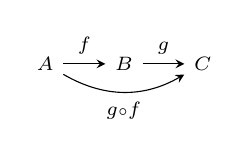
\begin{tikzpicture}[baseline=-0.7ex]
\node (A) {\(A\)};
\node (B) [right of=A] {\(B\)};
\node (C) [right of=B] {\(C\)};
\path[->]
(A) edge node[above]{\(f\)} (B)
(B) edge node[above]{\(g\)} (C)
(A) edge [bend right] node[below]{\(g{\scriptscriptstyle \circ} f\)} (C)
;
\end{tikzpicture}
when \(\cod f = \dom g\)
\end{quote}
%\(A\xrightarrow{f} B\xrightarrow{g}C\)

Identity axiom:
\begin{quote}
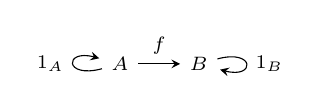
\begin{tikzpicture}[baseline=-0.7ex]
\node (A) {\(A\)};
\node (B) [right of=A] {\(B\)};
\path[->]
(A) edge node[above]{\(f\)} (B)
(A) edge [loop left] node[left]{\(1_A\)} (A)
(B) edge [loop right] node[right]{\(1_B\)} (B)
;
\end{tikzpicture}
with \(f1_A = f = 1_Bf\)
\end{quote}

Associative axiom:
\begin{quote}
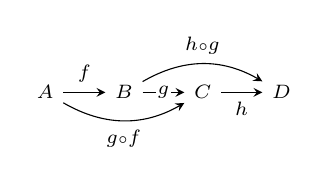
\begin{tikzpicture}[baseline=-0.7ex]
\node (A) {\(A\)};
\node (B) [right of=A] {\(B\)};
\node (C) [right of=B] {\(C\)};
\node (D) [right of=C] {\(D\)};
\path[->]
(A) edge node[above]{\(f\)} (B)
(A) edge [bend right] node[below]{\(g{\scriptscriptstyle \circ} f\)} (C)
;
\path[->](B) edge node[fill=white,inner sep=.5pt]{\(g\)} (C)
(B) edge [bend left] node[above]{\(h{\scriptscriptstyle \circ} g\)} (D)
;
\path[->]
(C) edge node[below]{\(h\)} (D)
;
\end{tikzpicture}
with \(h(gf) = (hg)f\)
\end{quote}
\end{frame}

\begin{frame}
\frametitle{Examples}
\begin{description}
\item[Set] Sets and functions
\item[Par] Sets and partial functions
\item[Rel] Sets and relations
\item[Grp] Groups and homomorphisms
\item[Rng] Rings and homomorphisms
\item[Vec] Vectors spaces and linear transformations
\item[Pre] Presets with \(A\to B\) when \(A\preceq B\) (ref, tra)
\item[Pos] Posets with \(A\to B\) when \(A\preceq B\) (also ant)
\item[Cat] Categories and {\em functors}
\item[2-Cat] Functors and {\em natural transformations}
\end{description}
\end{frame}

\begin{frame}
\frametitle{Arrow Properties}
Let \(\hom_\mathcal{A}(A,B) = \{f\colon A\to B\}\) be all arrows from \(A\) to \(B\)
in the category \(\mathcal{A}\),
a.k.a. \(\mathcal{A}[A,B]\) or \([A,B]\) sometimes \(B^A\).
\begin{description}
\item[epic] \(gf = hf\) implies \(g = h\)
\item[monic] \(fg = fh\) implies \(g = h\)
\item[bi] Both epic and monic
\item[section] \(s\colon A\to B\) and \(fs = 1_A\) for some \(f\)
\item[retraction] \(r\colon A\to B\) and \(rg = 1_B\) for some \(g\)
\item[iso] Both a section and retraction
\end{description}

%\begin{tikzpicture}
%\node (A) at (-1,1) {\(A\)};
%\node (B) at (1, 1) {\(B\)};
%\node (C) at (0, 0) {\(A/\ker f\)};
%\path[->] (A) edge node[above] {\(f\)}(B);
%\path[->] (A) edge (C);
%\path[->] (C) edge (B);
%\end{tikzpicture}
\end{frame}

\begin{frame}
\frametitle{Object Properties}
\begin{description}
\item[initial]\(hom(I,A)\) always has exactly on arrow
\item[terminal]\(hom(A,T)\) always has exactly on arrow
\item[zero] both initial and terminal
\item[sub] iso class of monos \(m\colon S\to A\)
\item[quotient] iso class of epis \(e\colon A\to Q\)
\item[FIT] 
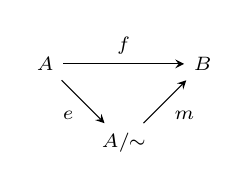
\begin{tikzpicture}[baseline=2ex]
\node (A) at (0,1) {\(A\)};
\node (B) at (2,1) {\(B\)};
\node (Q) at (1,0) {\(A/\!\!\sim\)};
\path[->] (A) edge node[above] {\(f\)} (B);
\path[->] (A) edge node[auto,swap] {\(e\)} (Q);
\path[->] (Q) edge node[auto,swap] {\(m\)} (B);
\end{tikzpicture}

\item[product]
\begin{tikzpicture}[baseline=5ex]
\node (T) at (0,2) {};
\node[circle,scale=0.3,fill=gray!5,draw] (P) at (0,1) {};
\node[circle,scale=0.3,fill=black,draw] (L) at (-1,0) {};
\node[circle,scale=0.3,fill=black,draw] (R) at (1, 0) {};
\path[->] (T) edge[dashed] (P);
\path[->] (P) edge (L);
\path[->] (P) edge (R);
\end{tikzpicture}
\item[coproduct]
\begin{tikzpicture}[baseline=-6ex]
\node (T) at (0,-2) {};
\node[circle,scale=0.3,fill=gray!5,draw] (P) at (0,-1) {};
\node[circle,scale=0.3,fill=black,draw] (L) at (-1,0) {};
\node[circle,scale=0.3,fill=black,draw] (R) at (1, 0) {};
\path[->] (P) edge[dashed] (T);
\path[->] (L) edge (P);
\path[->] (R) edge (P);
\end{tikzpicture}
\end{description}
\end{frame}

\begin{frame}
\frametitle{Productness}
A product \(A\xleftarrow{l}A\boxtimes B\xrightarrow{r}\) has the
property that
given \(C\xrightarrow{f}A\) and \(C\xrightarrow{g}B\) there
exists \(C\xrightarrow{h}A\boxtimes B\) such that
\(f = lh\) and \(g = rh\).
\begin{quote}
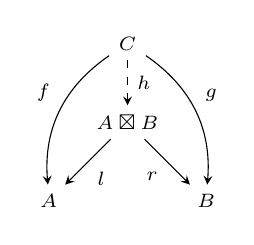
\begin{tikzpicture}
\node (C) at (0,2) {\(C\)};
\node (P) at (0,1) {\(A\boxtimes B\)};
\node (A) at (-1,0) {\(A\)};
\node (B) at (1,0) {\(B\)};
\path[->] (C) edge[dashed] node[right] {\(h\)} (P);
\path[->] (P) edge node[auto] {\(l\)} (A);
\path[->] (P) edge node[auto,swap] {\(r\)} (B);
\path[->] (C) edge[bend right] node[auto,swap] {\(f\)} (A);
\path[->] (C) edge[bend left] node[auto] {\(g\)}(B);
\end{tikzpicture}
\end{quote}
A product is an initial object in a certain category.
\begin{tabular}{|c|c|c|}
\hline 
Category & Symbol & Description \\ 
\hline 
Set & \(\times\) & Cartesian product \\ 
\hline 
Vec & \(\otimes\) & tensor product \\ 
\hline 
Pos & \(\wedge\) & join \\ 
\hline 
\end{tabular} 
\end{frame}

\begin{frame}
\frametitle{Functors and Natural Transformations}
A {\em functor} \(F\colon\mathcal{A}\to\mathcal{B}\) takes objects and
arrows of \(\mathcal{A}\) to objects and arrows of \(\mathcal{B}\) while
preserving the category structure:
if \(A\xrightarrow{f}B\) in \(\mathcal{A}\) then
\(FA\xrightarrow{Ff}FB\) in \(\mathcal{B}\) and
\begin{align*}
F1_A &= 1_{FA}\\
F(fg) &= (Ff)(Fg)\\
\end{align*}
A {\em natural transformation} \(\eta\colon F\to G\), where
\(F,G\colon\mathcal{A}\to\mathcal{B}\) are functors, takes
objects of \(\mathcal{A}\) to arrows of \(\mathcal{B}\) with 
\[G(f)\eta_A = \eta_BF(f)\]
when \(A\xrightarrow{f}B\).
\end{frame}

\begin{frame}
\frametitle{Double Dual in Vec}
Let \(V\) be a vector space and \(V^* = \hom(V,\mathbb{F})\) be its dual.
\newline
For \(T\in\hom(V, W)\) define
\(T^*\in\hom(W^*, V^*)\) by \[v(T^*w^*) = w^*(Tv).\] 
\newline
Call this functor \(D\). There is a natural transformation \(\eta\colon I\to D^2\)
given by \(\eta_V = V\to V^{**}\), \(\eta_V(v)v^* = v^*v\).
\begin{quote}
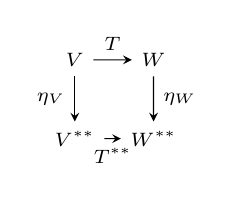
\begin{tikzpicture}[scale=1.2]
\node (V) at (0,2) {\(V\)};
\node (W) [right of=V] {\(W\)};
\node (Vdd) [below of=V] {\(V^{**}\)};
\node (Wdd) [below of=W] {\(W^{**}\)};
\path[->] (V) edge node[above] {\(T\)} (W);
\path[->] (V) edge node[left] {\(\eta_V\)} (Vdd);
\path[->] (W) edge node[right] {\(\eta_W\)} (Wdd);
\path[->] (Vdd) edge node[below] {\(T^{**}\)} (Wdd);
\end{tikzpicture}
\end{quote}
\end{frame}

\begin{frame}
\frametitle{Monads}
Given an endofunctor \(T\colon\mathcal{C}\to\mathcal{C}\), a {\em monad}
is a pair of natural transformations \(\nu\colon I\to T\) and \(\mu\colon T^2\to T\)
such that
\begin{quote}
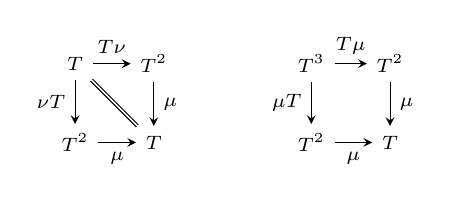
\begin{tikzpicture}
\node (T_) at (0,2) {\(T\)};
\node (T2_) [right of=T_] {\(T^2\)};
\node (TT_) [below of=T_] {\(T^2\)};
\node (T1_) [below of=T2_] {\(T\)};
\path[->] (T_) edge node[above] {\(T\nu\)} (T2_);
\path[->] (T_) edge node[left] {\(\nu T\)} (TT_);
\path[->] (TT_) edge node[below] {\(\mu\)} (T1_);
\path[->] (T2_) edge node[right] {\(\mu\)} (T1_);
\draw[double] (T_) -- (T1_);

\node (T3) at (3,2) {\(T^3\)};
\node (T2) [right of=T3] {\(T^2\)};
\node (TT) [below of=T3] {\(T^2\)};
\node (T) [below of=T2] {\(T\)};
\path[->] (T3) edge node[above] {\(T\mu\)} (T2);
\path[->] (T3) edge node[left] {\(\mu T\)} (TT);
\path[->] (TT) edge node[below] {\(\mu\)} (T);
\path[->] (T2) edge node[right] {\(\mu\)} (T);

\end{tikzpicture}
\end{quote}
commute, where the double line indicates identically equal.
Note \((T\nu)_A = T(\nu_A)\) and \((\nu T)_A = \nu_{TA}\).
\newline
The idea is that \(\nu\), aka {\em unit}, wraps up \(T\) and \(\mu\),
aka {\em lift},
acts on the wrapped up object. This provides a
mechanism to turn something that is not functional
into something that is.
\end{frame}

\begin{frame}[fragile]
\frametitle{Monad Example}
Suppose we had a library of error code returning functions like
\texttt{int f(double x, double* y)}. (Think GSL.)
we can define a class \texttt{unit} and function \texttt{lift} by
\begin{verbatim}
struct unit {
    int err;
    double val;
    unit(double x = 0, int e = 0) : err(e), val(x) {}
};
std::function<unit(unit)> 
lift(std::function<int(double,double*)> f) {
    return [f](unit x) { 
    	unit y;
    	y.err = x.err ? x.err : f(x.val, &y.val);
        return y;
    };
}
\end{verbatim}
\end{frame}

\begin{frame}[fragile]
\frametitle{Monad Use}
Now instead of 
\begin{verbatim}
err = f(x, &y)
if (err) { /* deal with it */ }
err = g(y, &z)
if (err) { /* deal with it */ }
\end{verbatim}
we can write
\begin{verbatim}
auto F = lift(f); auto G = lift(g);
unit z = G(F(unit(x)));
\end{verbatim}

\end{frame}

\end{document}